\documentclass[border=6pt]{standalone}
\usepackage[T1]{fontenc}
\usepackage{lmodern}
\usepackage{xcolor}
\usepackage{tikz}
\usetikzlibrary{arrows.meta}
\definecolor{NordBody}{HTML}{4C566A}
\definecolor{NordBlue}{HTML}{5E81AC}
\definecolor{NordPanel}{HTML}{ECEFF4}
\definecolor{NordRed}{HTML}{BF616A}
\definecolor{NordOrange}{HTML}{D08770}
\begin{document}
\begin{tabular}{c}
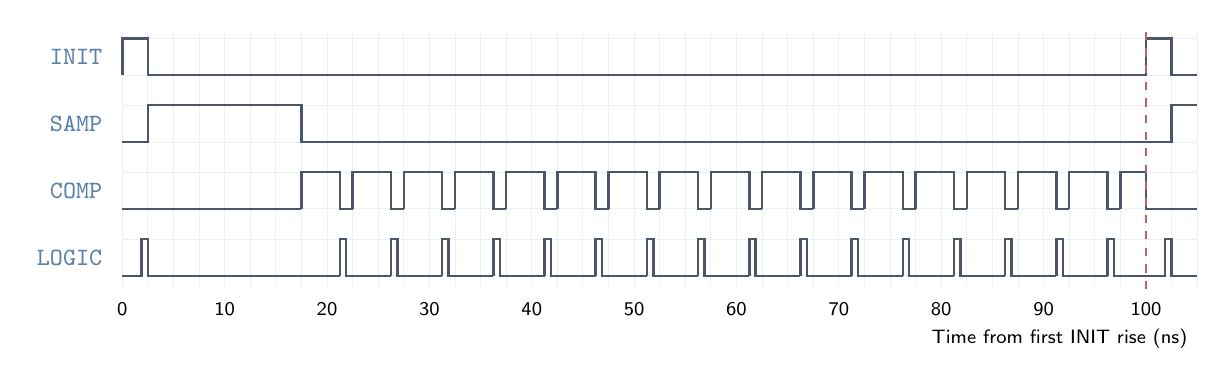
\begin{tikzpicture}[
  x=0.13cm,y=0.85cm,font=\sffamily\scriptsize,
  waveform/.style={draw=NordBody,line width=0.9pt},
  guide/.style={draw=NordPanel,line width=0.35pt}]
  \foreach \t in {0,2.5,...,105} {\draw[guide] (\t,-0.15) -- (\t,3.65);}
  \foreach \y/\name in {3/INIT,2/SAMP,1/COMP,0/LOGIC} {
    \draw[guide] (0,\y) -- (105,\y);
    \draw[guide] (0,{\y+0.55}) -- (105,{\y+0.55});
    \node[anchor=east,text=NordBlue,font=\ttfamily\bfseries\small] at (-1,\y+0.275) {\name};
  }
  \draw[waveform] (0,3) -- (0,3.55) -- (2.5,3.55) -- (2.5,3)
    -- (100,3) -- (100,3.55) -- (102.5,3.55) -- (102.5,3) -- (105,3);
  \draw[waveform] (0,2) -- (2.5,2) -- (2.5,2.55) -- (17.5,2.55)
    -- (17.5,2) -- (102.5,2) -- (102.5,2.55) -- (105,2.55);
  \draw[waveform] (0,1) -- (17.5,1);
  \foreach \k in {0,...,16} {
    \pgfmathsetmacro{\start}{17.5+5*\k}
    \pgfmathsetmacro{\stop}{min(\start+3.75,100)}
    \pgfmathsetmacro{\next}{min(\start+5,105)}
    \draw[waveform] (\start,1) -- (\start,1.55) -- (\stop,1.55)
      -- (\stop,1) -- (\next,1);
  }
  \draw[waveform] (102.5,1) -- (105,1);
  \draw[waveform] (0,0) -- (1.875,0) -- (1.875,0.55) -- (2.5,0.55)
    -- (2.5,0) -- (21.25,0);
  \foreach \k in {0,...,15} {
    \pgfmathsetmacro{\start}{21.25+5*\k}
    \pgfmathsetmacro{\stop}{\start+0.625}
    \pgfmathsetmacro{\next}{\start+5}
    \draw[waveform] (\start,0) -- (\start,0.55) -- (\stop,0.55)
      -- (\stop,0) -- (\next,0);
  }
  \draw[waveform] (101.25,0) -- (101.875,0) -- (101.875,0.55)
    -- (102.5,0.55) -- (102.5,0) -- (105,0);
  \draw[NordRed,dashed] (100,-0.2) -- (100,3.7);
  \foreach \t in {0,10,...,100} {\node[anchor=north] at (\t,-0.25) {\t};}
  \node[anchor=north east] at (105,-0.65) {Time from first INIT rise (ns)};
\end{tikzpicture}\\[5mm]
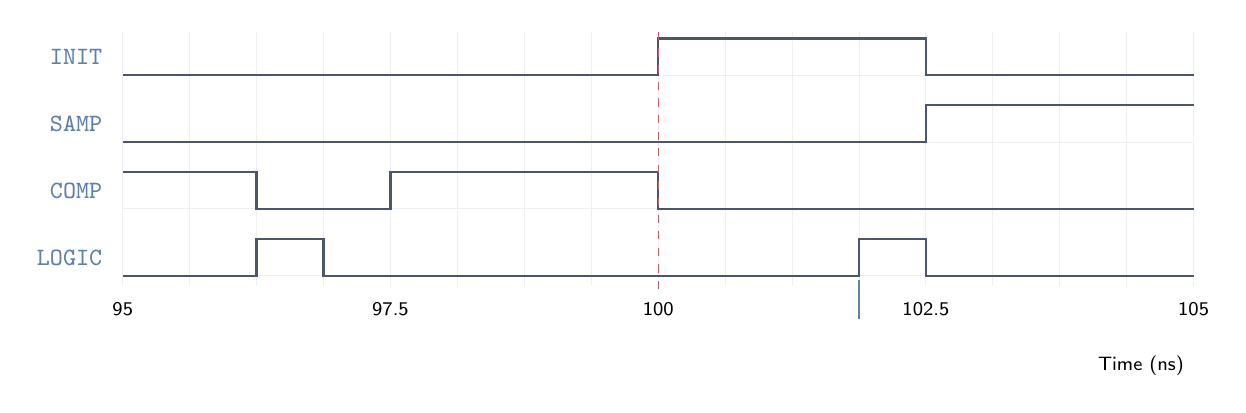
\begin{tikzpicture}[
  x=1.36cm,y=0.85cm,font=\sffamily\scriptsize,
  waveform/.style={draw=NordBody,line width=0.9pt},
  guide/.style={draw=NordPanel,line width=0.35pt}]
  % Coordinates here are time in ns minus 95 ns.
  \foreach \t in {0,0.625,...,10} {\draw[guide] (\t,-0.15) -- (\t,3.65);}
  \foreach \y/\name in {3/INIT,2/SAMP,1/COMP,0/LOGIC} {
    \draw[guide] (0,\y) -- (10,\y);
    \node[anchor=east,text=NordBlue,font=\ttfamily\bfseries\small] at (-0.1,\y+0.275) {\name};
  }
  \draw[waveform] (0,3) -- (5,3) -- (5,3.55) -- (7.5,3.55) -- (7.5,3) -- (10,3);
  \draw[waveform] (0,2) -- (7.5,2) -- (7.5,2.55) -- (10,2.55);
  \draw[waveform] (0,1.55) -- (1.25,1.55) -- (1.25,1) -- (2.5,1)
    -- (2.5,1.55) -- (5,1.55) -- (5,1) -- (10,1);
  \draw[waveform] (0,0) -- (1.25,0) -- (1.25,0.55) -- (1.875,0.55)
    -- (1.875,0) -- (6.875,0) -- (6.875,0.55) -- (7.5,0.55) -- (7.5,0) -- (10,0);
  \draw[NordRed,dashed] (5,-0.2) -- (5,3.7);
  \foreach \x/\label in {0/95,2.5/97.5,5/100,7.5/102.5,10/105}
    {\node[anchor=north] at (\x,-0.25) {\label};}
  \draw[NordBlue] (6.875,-0.06) -- (6.875,-0.65);
  \node[anchor=north east] at (10,-1.05) {Time (ns)};
\end{tikzpicture}
\end{tabular}
\end{document}
